% Options for packages loaded elsewhere
\PassOptionsToPackage{unicode}{hyperref}
\PassOptionsToPackage{hyphens}{url}
%
\documentclass[
]{article}
\usepackage{lmodern}
\usepackage{amssymb,amsmath}
\usepackage{ifxetex,ifluatex}
\ifnum 0\ifxetex 1\fi\ifluatex 1\fi=0 % if pdftex
  \usepackage[T1]{fontenc}
  \usepackage[utf8]{inputenc}
  \usepackage{textcomp} % provide euro and other symbols
\else % if luatex or xetex
  \usepackage{unicode-math}
  \defaultfontfeatures{Scale=MatchLowercase}
  \defaultfontfeatures[\rmfamily]{Ligatures=TeX,Scale=1}
\fi
% Use upquote if available, for straight quotes in verbatim environments
\IfFileExists{upquote.sty}{\usepackage{upquote}}{}
\IfFileExists{microtype.sty}{% use microtype if available
  \usepackage[]{microtype}
  \UseMicrotypeSet[protrusion]{basicmath} % disable protrusion for tt fonts
}{}
\makeatletter
\@ifundefined{KOMAClassName}{% if non-KOMA class
  \IfFileExists{parskip.sty}{%
    \usepackage{parskip}
  }{% else
    \setlength{\parindent}{0pt}
    \setlength{\parskip}{6pt plus 2pt minus 1pt}}
}{% if KOMA class
  \KOMAoptions{parskip=half}}
\makeatother
\usepackage{xcolor}
\IfFileExists{xurl.sty}{\usepackage{xurl}}{} % add URL line breaks if available
\IfFileExists{bookmark.sty}{\usepackage{bookmark}}{\usepackage{hyperref}}
\hypersetup{
  pdftitle={Statistical analysis in RStudio},
  hidelinks,
  pdfcreator={LaTeX via pandoc}}
\urlstyle{same} % disable monospaced font for URLs
\usepackage[margin=1in]{geometry}
\usepackage{longtable,booktabs}
% Correct order of tables after \paragraph or \subparagraph
\usepackage{etoolbox}
\makeatletter
\patchcmd\longtable{\par}{\if@noskipsec\mbox{}\fi\par}{}{}
\makeatother
% Allow footnotes in longtable head/foot
\IfFileExists{footnotehyper.sty}{\usepackage{footnotehyper}}{\usepackage{footnote}}
\makesavenoteenv{longtable}
\usepackage{graphicx,grffile}
\makeatletter
\def\maxwidth{\ifdim\Gin@nat@width>\linewidth\linewidth\else\Gin@nat@width\fi}
\def\maxheight{\ifdim\Gin@nat@height>\textheight\textheight\else\Gin@nat@height\fi}
\makeatother
% Scale images if necessary, so that they will not overflow the page
% margins by default, and it is still possible to overwrite the defaults
% using explicit options in \includegraphics[width, height, ...]{}
\setkeys{Gin}{width=\maxwidth,height=\maxheight,keepaspectratio}
% Set default figure placement to htbp
\makeatletter
\def\fps@figure{htbp}
\makeatother
\setlength{\emergencystretch}{3em} % prevent overfull lines
\providecommand{\tightlist}{%
  \setlength{\itemsep}{0pt}\setlength{\parskip}{0pt}}
\setcounter{secnumdepth}{5}
\usepackage{subfig}

\title{Statistical analysis in RStudio}
\author{}
\date{\vspace{-2.5em}}

\begin{document}
\maketitle

{
\setcounter{tocdepth}{2}
\tableofcontents
}
\hypertarget{abstact}{%
\subsubsection{Abstact}\label{abstact}}

\hypertarget{introduction}{%
\section{INTRODUCTION}\label{introduction}}

The main objective of statistical analysis is to find the correlation
and Trends of seal abundance using the serial dataset.

Firstly we will download the data and convert it into a csv file and
then import data into R studio after importing data We will read the
data and convert the data into data frame Which will import data into
rows and columns. If we check the head of data we can find There are 5
columns 210 observations.

\begin{itemize}
\tightlist
\item
  The first column represents the year, each row consists of the year
  from 2007 to 2010.
\item
  The second column represents the month of a specific year; there are
  15 unique variables if it presents the month of a particular Year.
\item
  The third column represents a site which consists of 7 unique
  variables A,B,C,D,Split and Wall.
\item
  The fourth column represents species which have true unique species
  Harbour and grey.
\item
  The final column represents the average count of each species in a
  particular year year and month each variable has a unique count value.
\end{itemize}

\begin{longtable}[]{@{}llllr@{}}
\toprule
Summer & Year.Month & Site & Species & average.count\tabularnewline
\midrule
\endhead
summer-2007 & 2007.Jun & A & HARBOUR & 14.1\tabularnewline
summer-2007 & 2007.Jun & B & HARBOUR & 0.3\tabularnewline
summer-2007 & 2007.Jun & C & HARBOUR & 14.7\tabularnewline
summer-2007 & 2007.Jun & Spit & HARBOUR & 0.1\tabularnewline
summer-2007 & 2007.Jun & Wall & HARBOUR & 0.7\tabularnewline
summer-2007 & 2007.Jun & D & HARBOUR & 0.0\tabularnewline
\bottomrule
\end{longtable}

\begin{verbatim}
## 'data.frame':    210 obs. of  5 variables:
##  $ Summer       : chr  "summer-2007" "summer-2007" "summer-2007" "summer-2007" ...
##  $ Year.Month   : chr  "2007.Jun" "2007.Jun" "2007.Jun" "2007.Jun" ...
##  $ Site         : chr  "A" "B" "C" "Spit" ...
##  $ Species      : chr  "HARBOUR" "HARBOUR" "HARBOUR" "HARBOUR" ...
##  $ average.count: num  14.1 0.3 14.7 0.1 0.7 0 0 0.3 0 2.6 ...
\end{verbatim}

\hypertarget{materials-and-methods}{%
\section{MATERIALS AND METHODS}\label{materials-and-methods}}

On this section we will use various methods for the statistical analysis
and explore the data which will help to understand the relationship
between dependent and independent variables. Before proceeding further
if we see the data set we can see that only column has numerical values
which we will be considering to use for our analysis, Moving into deep
observation, the Average count cosist of each numerical value which
represents the average count of seals presents in particular year an
month. In addition considering the observation it can be identified for
two species which is Grey and Harbor. We can say that the average count
is quiet dependent for each of rows and though each of the row is quiet
responsible of the analysis therefore in order to explore in the
detailed way we can run some normality test.

\hypertarget{normality-test}{%
\subsection{Normality Test}\label{normality-test}}

After checking rows and columns of data, it can be easily identified
that only the average.count data column has numerical value. If we check
the normality of the average.count column using the qqnorm()
function,The Below visualization data represents the relationship
between the theoretical and sample quantities which derive the plotted
data is distinctly curved and determines that the data is not normal.

\hypertarget{qqnorm-test}{%
\subsubsection{QQNORM TEST}\label{qqnorm-test}}

qqnorm is generic function in r that produces which helps to generate
Quantile plot of the y values. The x plot consists of theoretical values
where as the y plot consists of sample quantities. A Quantile-Quantify
(Q-Q) plot is a scatter plot comparing the fitted and empirical
distributions in terms of the dimensional values of the variable (i.e.,
empirical quantifies)(Vito Ricco,p.4).

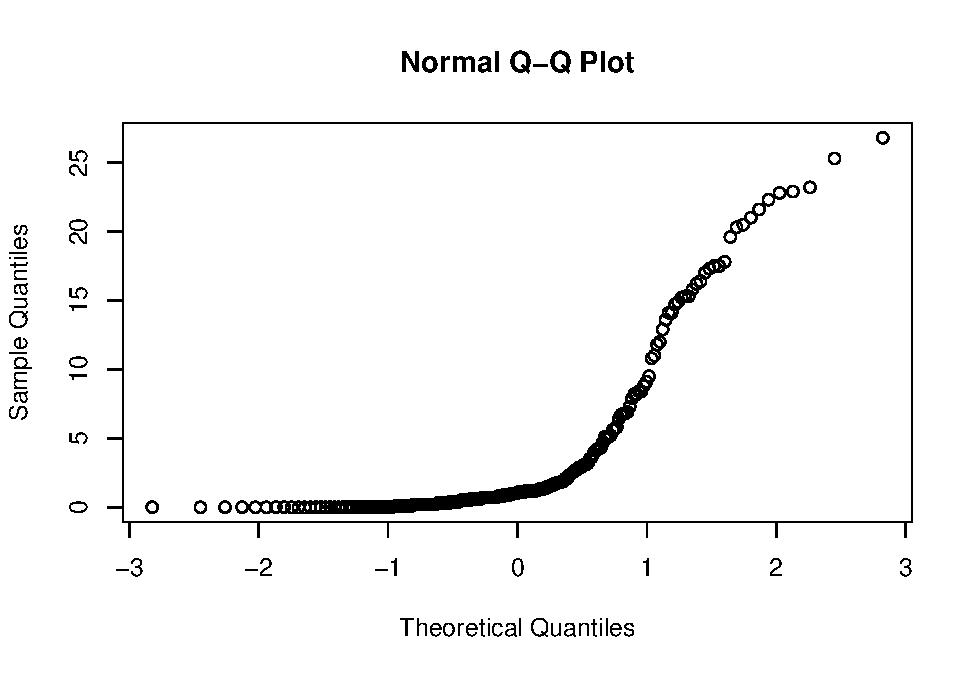
\includegraphics{Statistical-analysis-in-RStudio_files/figure-latex/unnamed-chunk-4-1.pdf}

While finding out that data is not normal in normality test using qqnorm
function, if we run the same test using shapiro.test() function, The
p-value is Greater than 0.01 we can say that it then all hypothesis is
not rejected Data is not significantly distributed therefore we have to
perform non parametric test.

\hypertarget{shapiro-test}{%
\subsubsection{shapiro Test}\label{shapiro-test}}

Shaprio Normailty test is used to find whether the data is fit for the
normal distribution This test was the first test that was able to detect
departures from normality due to either skewness or kurtosis, or both
(Althouse et al., 1998)(Nornadiah Mohd Razali and Bee Wah Yap ,p.25).

When we run the shaprio test for average count we can see that the p
value is 2.2 and the value of w is 0.67. Thus this test will reject the
normality.Since the data is not significant,in order to find out The
number of seals are significantly different for each year plot the data
of average count of number of seals for each year but before that we
have to change the data type of the first four columns into factors.

If we change the data type we get to know that

\begin{itemize}
\tightlist
\item
  The first column consist of four factor i.e 2007 till 2010
\item
  The Second column consists of 15 factor each factor is month of each
  year.
\item
  The Third column consists of seven factor, each factor has considered
  as the different sites of the species.
\item
  The Fourth Factor consists of two factor each factor is unique
  species.
\item
  The Final column is to be left over, as it has numerical data type and
  represents each unique counts for particular year and month.
\end{itemize}

As we have seen that, after changing the data type we can find that the
summer column has four factor levels, Year. month column has 15 factor
levels, the site column as 7 factor level and and the species column two
factor levels. Therefore we can check now how much average count of
species is there in each year which will be helpful to analyse the
normality of data.

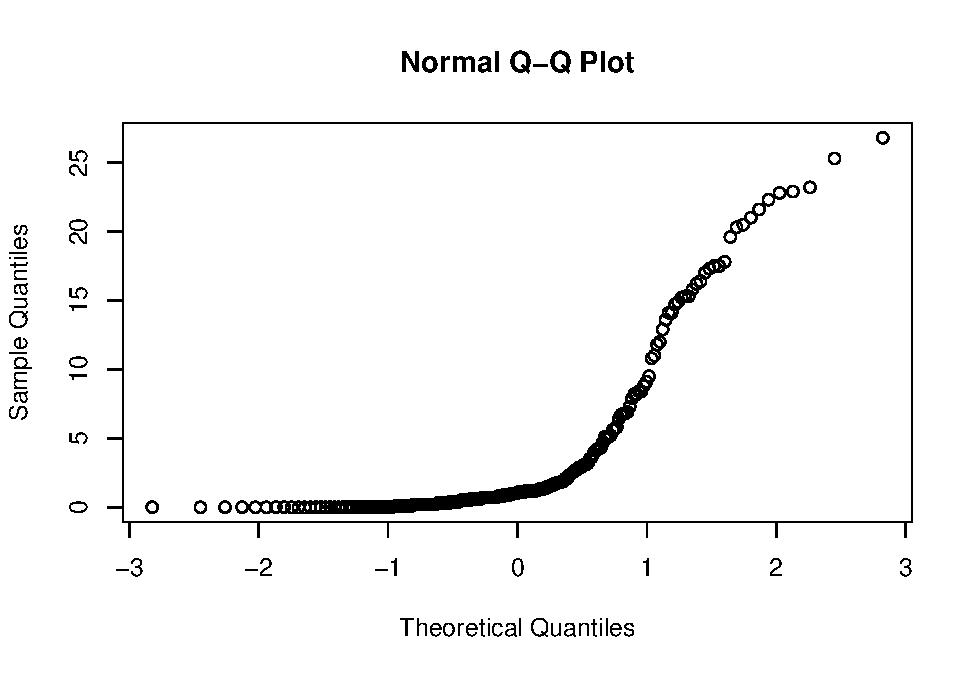
\includegraphics{Statistical-analysis-in-RStudio_files/figure-latex/unnamed-chunk-5-1.pdf}
In the above graph if we can see the the average count of species is
highest in 2009 and followed by 2010 where as the least count can be
seen in the year 2008 but visualizing the plot we can cannot consider
the changes are significant or not.

In order to find out this we can transfer some non parametric test like
kruskal Wallis rank sum test Which help us to determine the overall
correlation and statistical Association for data by providing a
chi-squared interpretation and a p-value.

\hypertarget{kruskal-wallis-test}{%
\subsubsection{Kruskal-Wallis Test}\label{kruskal-wallis-test}}

Kruskal Wallis Test is Considered as Non-Primitive test and an
alternative of Test.It is also called as One way ANNOVA test as the is
performed by different individual groups.They are considered as non-
primitive test because

the non-parametric tests are less powerful than their parametric
counterparts,i.e.~a parametric test is more likely to detect a genuine
effect in the data , if there is one, than a non-parametric test
(TEODORA H. MEHOTCHEVA,p.3).

In order to perform the Krukals-wallis test, we need to use the
kruskal.test() function.

\begin{verbatim}
## [1] 0.1006759
\end{verbatim}

Firstly, if we explore the overall difference between all the variables
we can see that The p-value is 0.10 and chi-squared value is 6.23 which
is greater than the normality distribution, thus we can say that it
There is no significant difference between the groups and considering
the the data we can also see that the data is not homogeneous.Yet, we
know there is difference but we don't know where it is.Therefore, In
order to explore this into more detail to find out that the pairs of
groups are different or not, will use pairwise willox test For comparing
different group levels for multiple testing.

\hypertarget{pairwise-wilocx-test}{%
\subsubsection{Pairwise wilocx Test}\label{pairwise-wilocx-test}}

Pairwise wilocx test is also a non-primitive test which uses the
multiple distributions or repetitive distributions where two or more
than two observation is considered to the test. This test helps to test
the significant distibtions of a group to derive the paticluar group
lies in normality or not.

Considering the the pairwise solution below for the average count and
the year group in order to find the data is significantly distributed or
not.

\begin{longtable}[]{@{}lrrr@{}}
\toprule
& 2007 & 2008 & 2009\tabularnewline
\midrule
\endhead
2008 & 0.8933132 & NA & NA\tabularnewline
2009 & 0.2023815 & 0.4280243 & NA\tabularnewline
2010 & 0.4280243 & 0.6385207 & 0.8933132\tabularnewline
\bottomrule
\end{longtable}

In the above test we can see that the P value for significant years is
quite normal. further, providing an adjustment method we can avoid the
false positive results in order to see more accuracy.

\begin{longtable}[]{@{}lrrr@{}}
\toprule
& 2007 & 2008 & 2009\tabularnewline
\midrule
\endhead
2008 & 0.5359879 & NA & NA\tabularnewline
2009 & 0.1730807 & 0.1730807 & NA\tabularnewline
2010 & 0.1730807 & 0.3192604 & 0.7529974\tabularnewline
\bottomrule
\end{longtable}

In the above test we can see that the adjusted P value is greater than
0.05, this shows that your value is not significant. In order to
understand it with more clarity if we plot our data we can see that
there was a significant difference between 2010 and 2007, we can see
that the highest number of seals were counted in 2010. Also we can see
that in 2007.

There were some high counts of seal, but in the previous bar graph it
was suggested that there was a big significant difference between 2007
and 2010. From this we can say that the statistical tests were more
accurate and help us to find the significant errors which were present
in data.

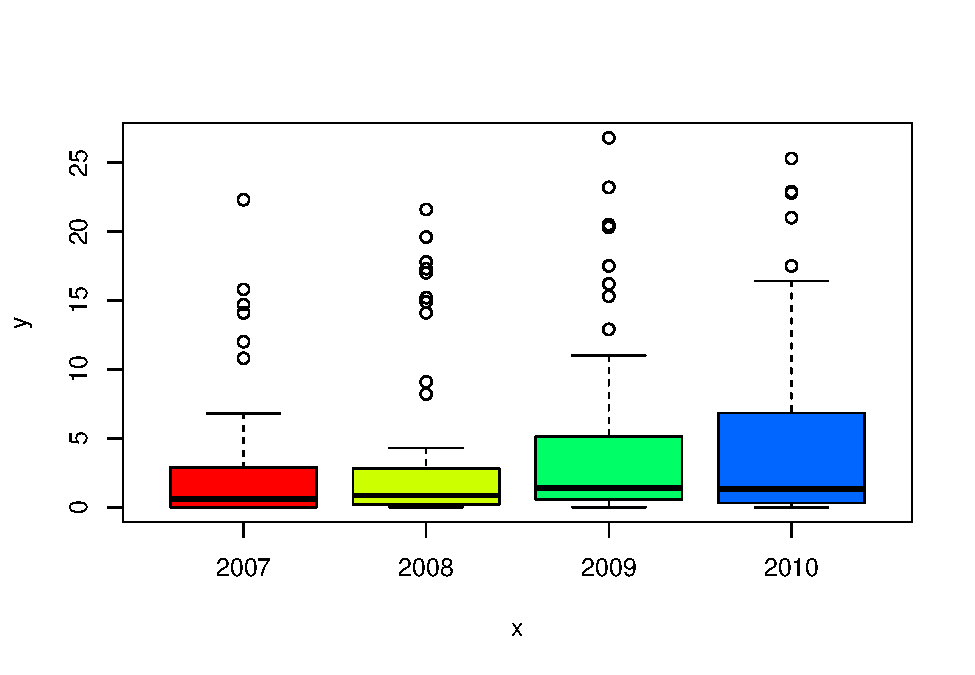
\includegraphics{Statistical-analysis-in-RStudio_files/figure-latex/unnamed-chunk-9-1.pdf}
After this we can check the presence of the seals for each month in a
particular year. We might be able to explore the difference for the
presence of seals in each month of the year.

The plot below shows the values of average count for each month of
particular year.We can see that in 2009 Aug,the number of species were
counted the most and in 2010 Sep the species were counted the least. But
in order to find significant relationship we need to explore the data
and run test accordingly.

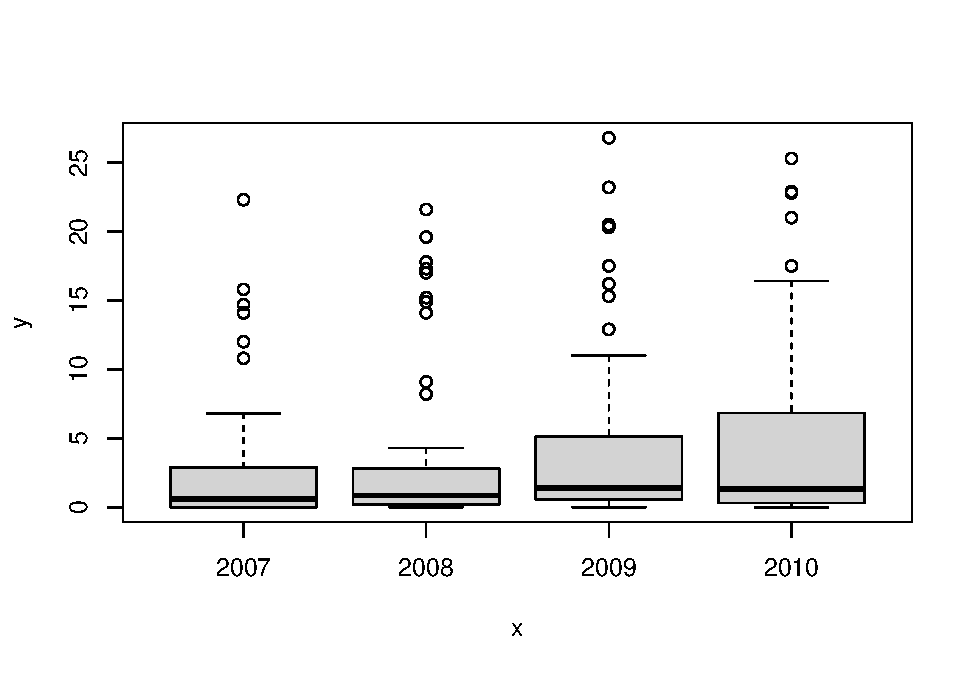
\includegraphics{Statistical-analysis-in-RStudio_files/figure-latex/unnamed-chunk-10-1.pdf}

\hypertarget{normality-test-for-each-month}{%
\subsection{Normality Test For Each
month}\label{normality-test-for-each-month}}

If we consider the year 2007, we can see that there is no significant
difference between different months.The p-value is 0.51 and the adjusted
p-value is than 0.62. Considering the normality, we have to explore for
the each year in order to find out if the data is significant or not not
in every year.

\begin{verbatim}
## [1] 0.5191072
\end{verbatim}

\begin{longtable}[]{@{}lrr@{}}
\toprule
& 2007.Aug & 2007.Jul\tabularnewline
\midrule
\endhead
2007.Jul & 0.6273101 & NA\tabularnewline
2007.Jun & 0.6273101 & 0.6273101\tabularnewline
\bottomrule
\end{longtable}

If we consider the year 2008, we can see that there is no significant
difference between different months.The p-vaule for kruskal test is 0.8
and the adjusted p-values is 0.93.Further, we need to check for 2009 and
2010.

\begin{verbatim}
## [1] 0.8349213
\end{verbatim}

\begin{longtable}[]{@{}lrrr@{}}
\toprule
& 2008.Aug & 2008.Jul & 2008.Jun\tabularnewline
\midrule
\endhead
2008.Jul & 0.9263274 & NA & NA\tabularnewline
2008.Jun & 0.9263274 & 0.9263274 & NA\tabularnewline
2008.Sep & 0.9263274 & 0.9263274 & 0.9263274\tabularnewline
\bottomrule
\end{longtable}

If we consider the year 2009, we can see that there is no significant
difference between different months. The p-value is 0.93 and the
adjusted p-value is 1. We can see that until now we didnot find any
significant differnce, lets check the the test of 2010.

\begin{verbatim}
## [1] 0.9359747
\end{verbatim}

\begin{longtable}[]{@{}lrrr@{}}
\toprule
& 2009.Aug & 2009.Jul & 2009.Jun\tabularnewline
\midrule
\endhead
2009.Jul & 1 & NA & NA\tabularnewline
2009.Jun & 1 & 1 & NA\tabularnewline
2009.Sep & 1 & 1 & 1\tabularnewline
\bottomrule
\end{longtable}

If we consider the year 2010, we can see that there is no significant
difference between different months. the p-value of the krukal test is
0.4 and the adjusted p-vaues varies from year to year, thus the
normality test for each month can be considered as the significant
difference therefore we can consider the normailty of each year.

\begin{verbatim}
## [1] 0.4752711
\end{verbatim}

\begin{longtable}[]{@{}lrrr@{}}
\toprule
& 2010.Aug & 2010.Jul & 2010.Jun\tabularnewline
\midrule
\endhead
2010.Jul & 0.7546306 & NA & NA\tabularnewline
2010.Jun & 0.5976528 & 0.9629236 & NA\tabularnewline
2010.Sep & 0.9629236 & 0.5976528 & 0.5976528\tabularnewline
\bottomrule
\end{longtable}

We have seen above the normality test also did not perform very well for
each month but we have seen that there should be a significant
difference in the data. So we will try to explore the Species group in
order to find the normality of derivatives.

\hypertarget{normality-test-for-species}{%
\subsection{Normality test for
Species}\label{normality-test-for-species}}

Considering the data and previous stats we found that there were no
significant difference for each month but in order to get detailed
information about the species we can check the count of each type of
species and find out the non-significant relationship of the data .

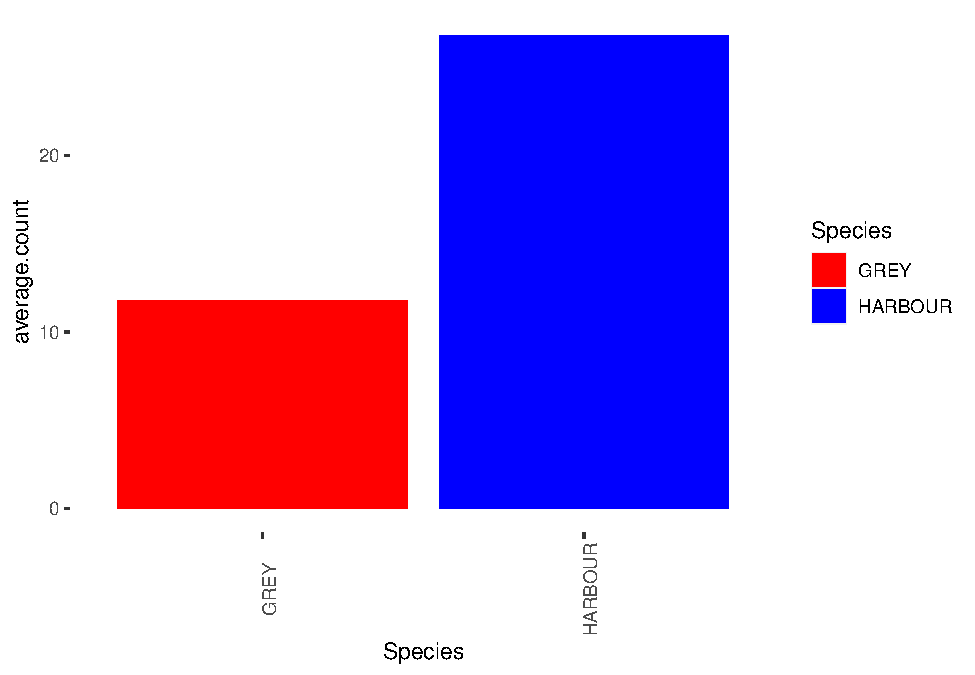
\includegraphics{Statistical-analysis-in-RStudio_files/figure-latex/unnamed-chunk-19-1.pdf}

As we had seen the above graph about the average count of the harbor
species are very much than the grey species.We can say that the Harbor
species are more common than the grey species, using the kruskal test we
can find out the difference between each species.

\begin{verbatim}
## [1] 1.561916e-05
\end{verbatim}

\begin{longtable}[]{@{}lr@{}}
\toprule
& GREY\tabularnewline
\midrule
\endhead
HARBOUR & 1.57e-05\tabularnewline
\bottomrule
\end{longtable}

After performing the test we can easily see the p values is greater than
0.01 and after plotting the below graph we can say that the Harbour
seals population are more comparatively grey. In other way, it can be
derived that the harbor seals are more significantly common than the
grey species.

Also, we can explore data in more detailed way in order to find out
significant difference of species for each year.

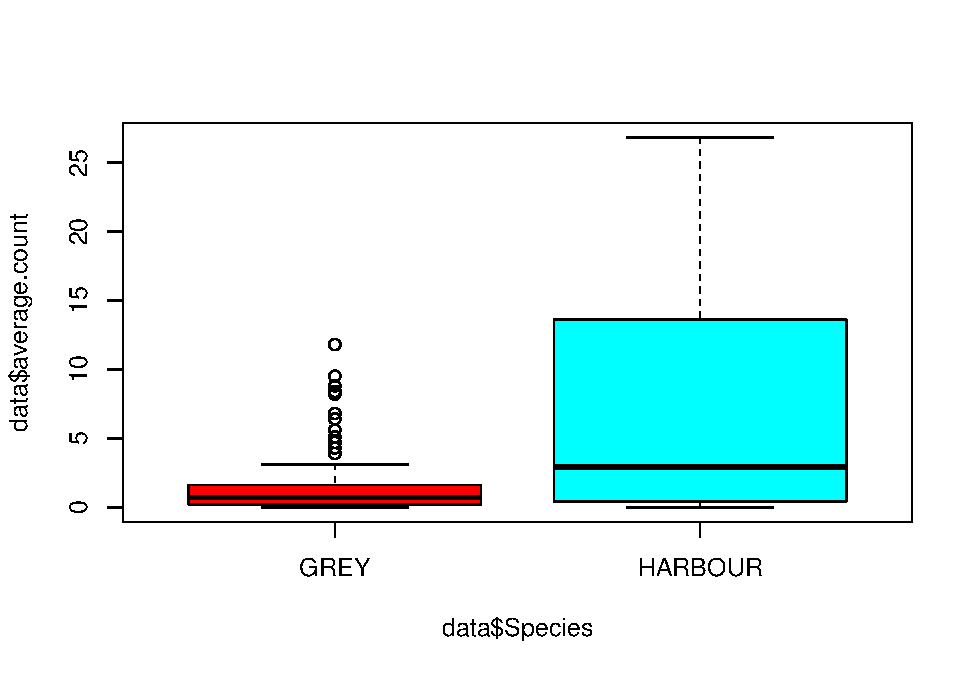
\includegraphics{Statistical-analysis-in-RStudio_files/figure-latex/unnamed-chunk-22-1.pdf}

If we look at the below stats, we can clearly see the p-value for 2007
year is 0.09 and adjusted p-value is 0.07 also greater than the
significant value which derives there is slightest significance
difference in the Species. However this test will fail considering the
significant difference of normality test.

\begin{verbatim}
## [1] 0.06938051
\end{verbatim}

\begin{longtable}[]{@{}lr@{}}
\toprule
& GREY\tabularnewline
\midrule
\endhead
HARBOUR & 0.0713513\tabularnewline
\bottomrule
\end{longtable}

Again, If we look at the below stats, we can clearly see the p-value for
2008 year is 0.09 and adjusted p-value is 0.10 which is greater than
significant value which derives the group is not in range of normailty
and we have to consider it as a failed test.

\begin{verbatim}
## [1] 0.09866302
\end{verbatim}

\begin{longtable}[]{@{}lr@{}}
\toprule
& GREY\tabularnewline
\midrule
\endhead
HARBOUR & 0.100351\tabularnewline
\bottomrule
\end{longtable}

If we look at the below stats, we can clearly see the p-value for 2009
year is to 0.001 and adjusted p-value is also 0.001 which derives there
is significance difference in the Species.Therefore we can say that the
data is normaly distributed in the year 2009.

\begin{verbatim}
## [1] 0.001307411
\end{verbatim}

\begin{longtable}[]{@{}lr@{}}
\toprule
& GREY\tabularnewline
\midrule
\endhead
HARBOUR & 0.0013452\tabularnewline
\bottomrule
\end{longtable}

Finally, If we look at the below stats, we can clearly see the p-value
for 2010 year is 0.04 and adjusted p-value is is 0.04 which derives
there is significance difference in the Species. Therfore we can say
that the data is normaly distibuted in the year 2010

\begin{verbatim}
## [1] 0.04234657
\end{verbatim}

\begin{longtable}[]{@{}lr@{}}
\toprule
& GREY\tabularnewline
\midrule
\endhead
HARBOUR & 0.0431888\tabularnewline
\bottomrule
\end{longtable}

From this we can easily say that in 2007 and 2008 the population of
species were not significantly different where as in 2009 and 2010 we
can say that the population is significantly different from other.By
this we can say that in the year 2009 and 2010 the data is significantly
distributed and is normalized.

Therefore from here we need to calculate the error in order to find the
out better results and improve the performance but before that we can
check the population of individual species for particular month and
further we can develop the error bars after calculating the error .

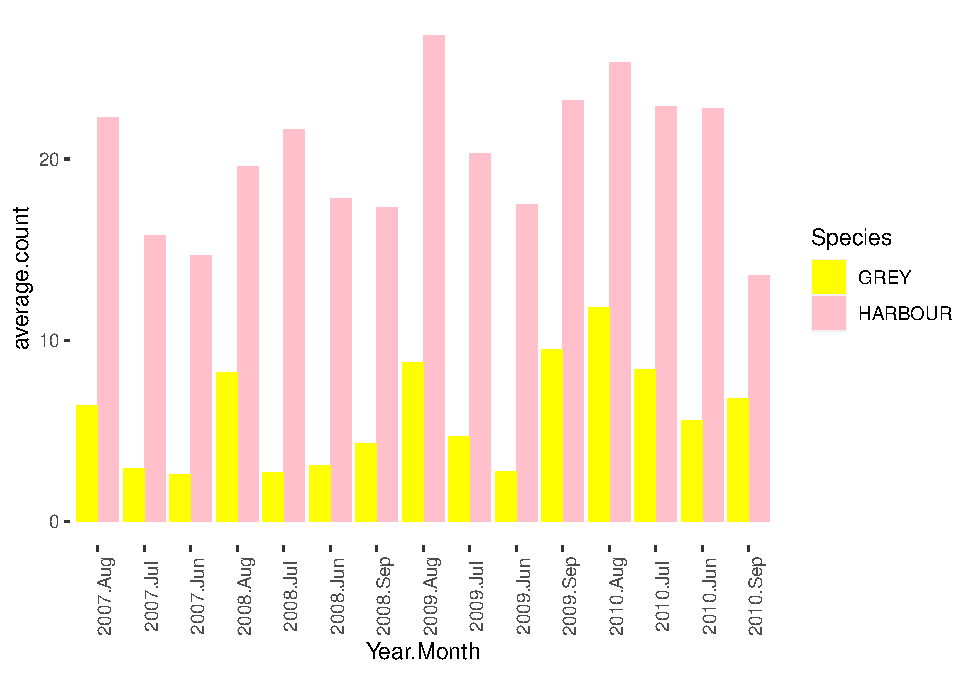
\includegraphics{Statistical-analysis-in-RStudio_files/figure-latex/unnamed-chunk-31-1.pdf}

If you look at the graph of average count of each species in a
particular month everywhere we can see that the existence of herbal
species are way more than the gray species. Therefore we can say that
the herbal species are more common than the gray species.In order to
find the significant differences between the species we need to find the
error species for particular month in each year using SummarySE()
function.

\begin{longtable}[]{@{}llrrrrr@{}}
\toprule
Year.Month & Species & N & average.count & sd & se & ci\tabularnewline
\midrule
\endhead
2007.Aug & GREY & 7 & 1.2857143 & 2.2886885 & 0.8650430 &
2.1166839\tabularnewline
2007.Aug & HARBOUR & 7 & 6.3428571 & 8.2679818 & 3.1250034 &
7.6466079\tabularnewline
2007.Jul & GREY & 7 & 0.8714286 & 1.2051477 & 0.4555030 &
1.1145757\tabularnewline
2007.Jul & HARBOUR & 7 & 5.1714286 & 6.0939080 & 2.3032807 &
5.6359249\tabularnewline
2007.Jun & GREY & 7 & 0.7142857 & 0.9599107 & 0.3628121 &
0.8877693\tabularnewline
2007.Jun & HARBOUR & 7 & 4.2714286 & 6.9254878 & 2.6175883 &
6.4050079\tabularnewline
\bottomrule
\end{longtable}

The Below Graph represents the standard deviation of each of the species
in particular months in a years. Considering the graph we can see that
the In August 2010 the standard deviation seems to be very far from the
mean value but in 2009 June and July, The SD values are very close to
with mean value.

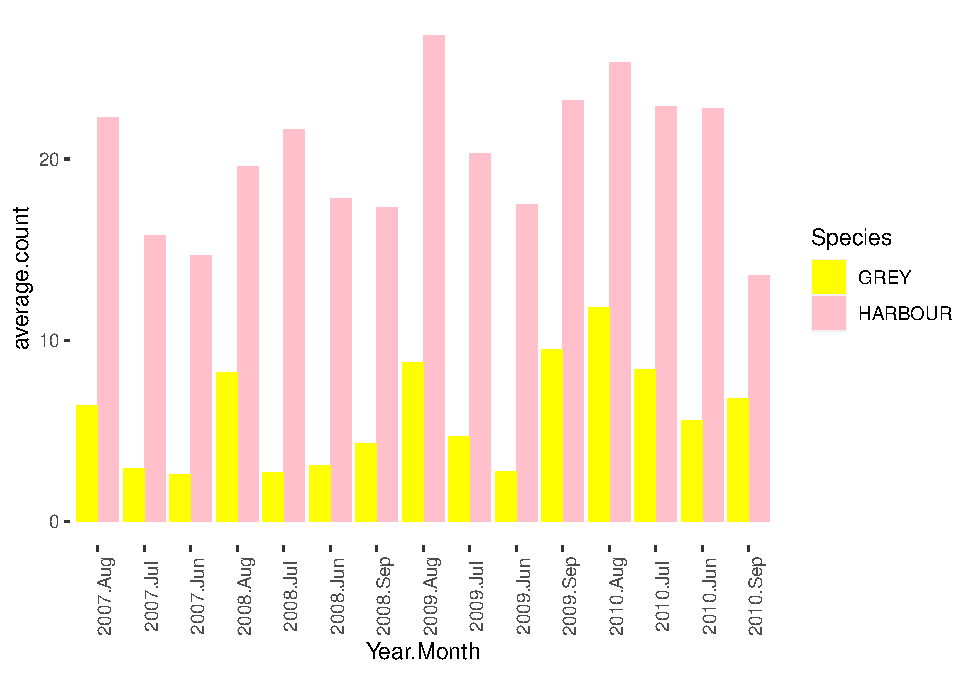
\includegraphics{Statistical-analysis-in-RStudio_files/figure-latex/unnamed-chunk-33-1.pdf}

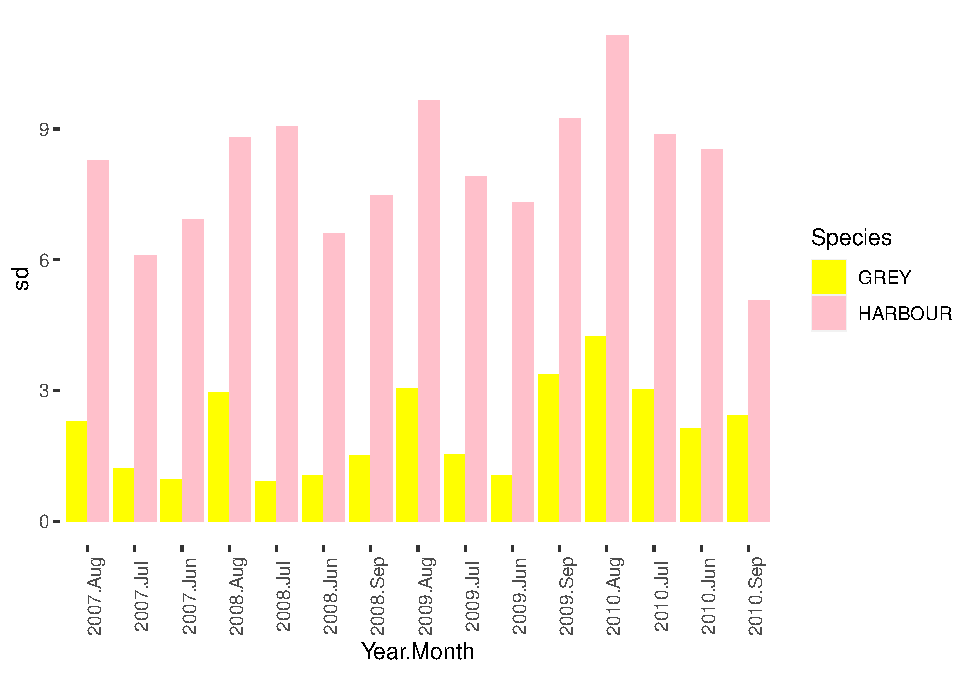
\includegraphics{Statistical-analysis-in-RStudio_files/figure-latex/unnamed-chunk-34-1.pdf}

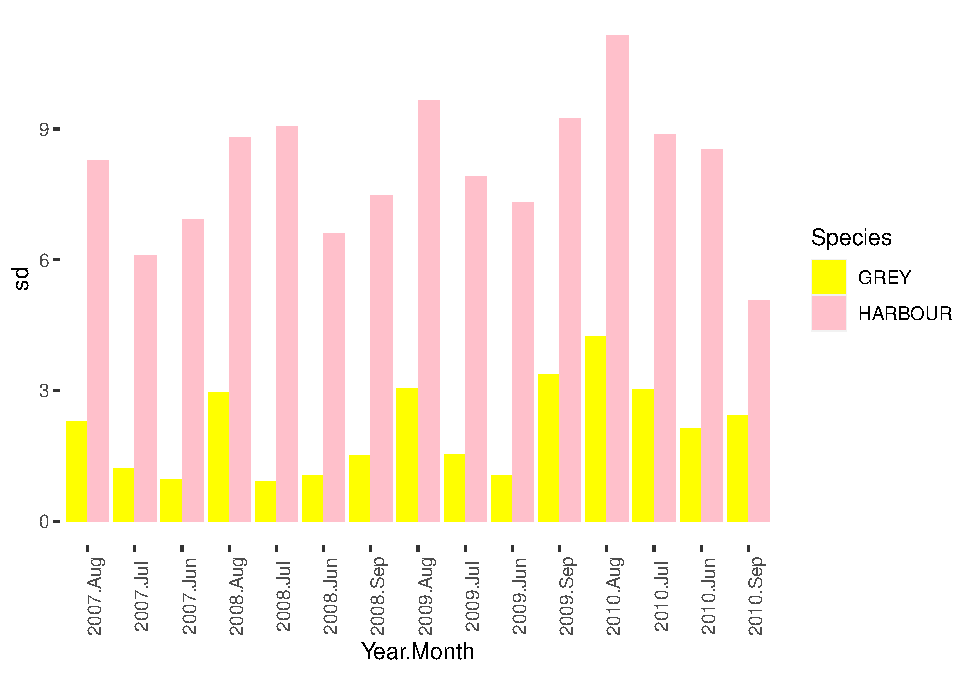
\includegraphics{Statistical-analysis-in-RStudio_files/figure-latex/unnamed-chunk-35-1.pdf}

If we check summary data we can find that the date of it consists of
count, mean, standard deviation, standard error of mean and confidence
interval. in order to find more detailed information we can plot the
significant errors graph using ggplot2 in order to find significant
difference between each species

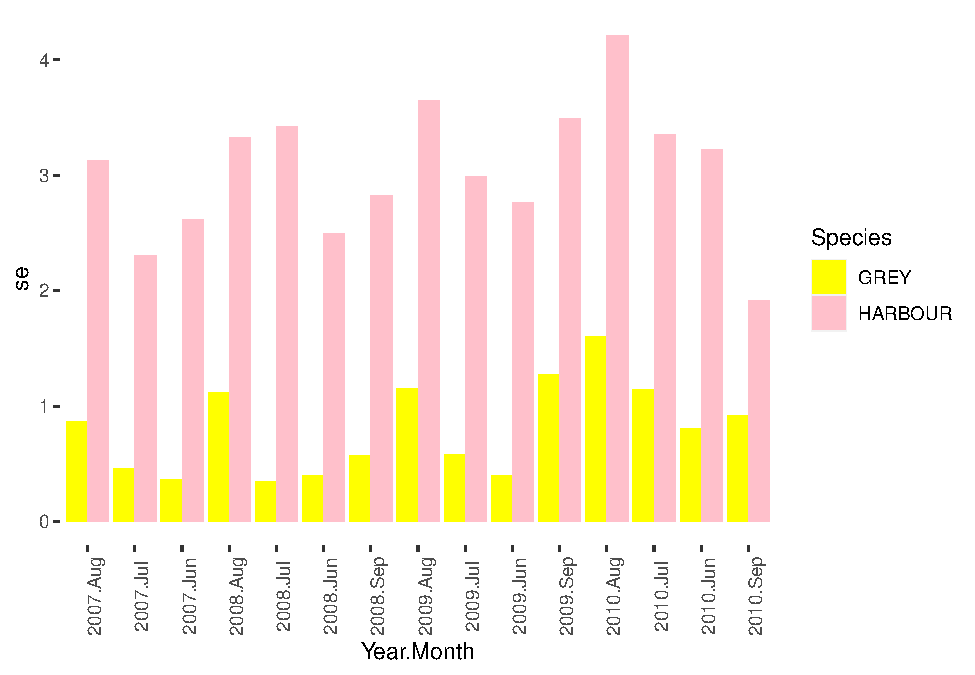
\includegraphics{Statistical-analysis-in-RStudio_files/figure-latex/unnamed-chunk-36-1.pdf}

Considering the above graph clearly shows that the graph provides an
error bar which significantly shows how each species is using standard
error. This clearly signifies difference species for a particular month.

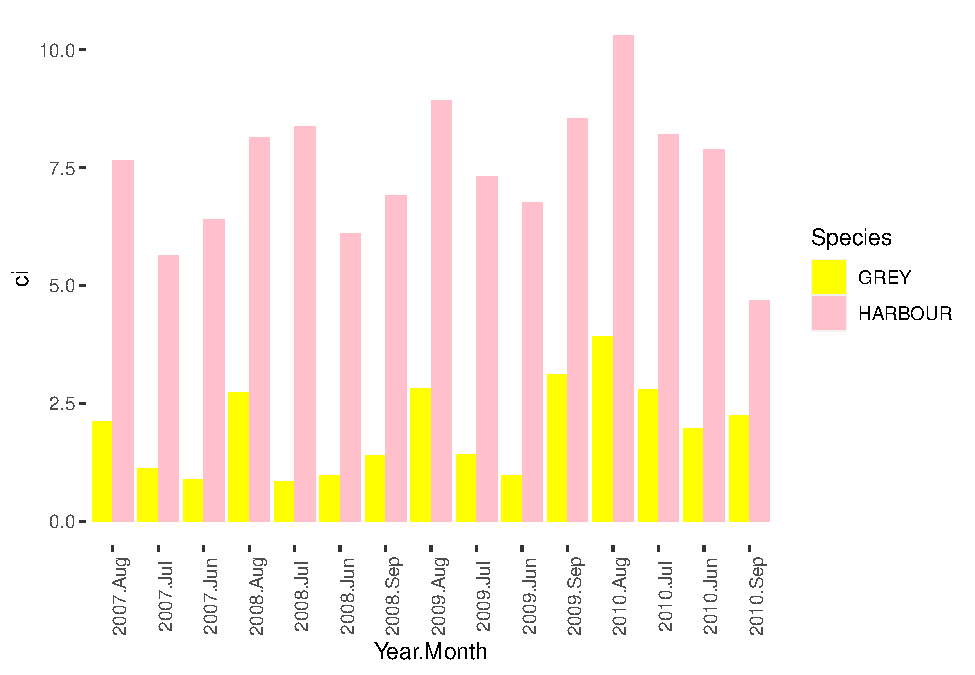
\includegraphics{Statistical-analysis-in-RStudio_files/figure-latex/unnamed-chunk-37-1.pdf}

\hypertarget{results}{%
\section{RESULTS}\label{results}}

In the above test, we have analysed the significant difference between
the species and the count values. We have different nominal variables
and only one measure of variables, however we are able to identify
non-significant values of the population of seals over time.\\
Moreover, when comparing data according to the year wise, we found out
that the highest seal was obtained in 2010 and there were high counts in
summer 2007. But they also found out that the levels of variance in the
data particularly word not explored. Therefore we started exploring data
for each month in a year in order to find out the presence of seals, but
the test suggested that there is no significant difference and different
months for each year. Moreover, Started analysing particular species for
each year. Initially we had seen that the harbour seals species are more
common than grey sea species, after that we found out 2009 and 10 the
data appeared to be more significant 2007 and 2008 the data was slightly
significant. After that, we calculated the standard error, and
visualised the data which represented how the variables are using
standard errors.

By summing up, we can say that the data is well explored, analysed and
ready to be processed for modelling which will help to give better
results for prediction.

\hypertarget{discussion}{%
\section{DISCUSSION}\label{discussion}}

In the above data, We were able to successfully explore and analyse and
find out the normality distribution of existence for both the species.
According to the non parametric test, the most common use of Kruskal
Wallis Test is when the data has one nominal variable and one
measurement variable but test does not assume that a data han is well
distributed and completely align for two parameters which can be mean
and standard deviation and also it is called as one way
anova(Biostathandbook, One Way Annovas). also this test assumes that the
null hypothesis of mean groups are same. therefore if distribution
groups are same, the Kruskal wallis test will not show a significant
difference in their distribution. Yet, the test does not considered that
the data are normally distributed, which can be a big advantage but 800
data has different groups different variants the test will give
inaccurate result. Therefore, if the distribution is different and
variant is different we can use anova test for accurate results

\hypertarget{references}{%
\subsubsection{REFERENCES}\label{references}}

\begin{itemize}
\item
  FITTING DISTRIBUTIONS WITH R by Mr Vito Ricci.\\
  Avialable from:
  \url{https://mran.revolutionanalytics.com/snapshot/2015-11-22/doc/contrib/Ricci-distributions-en.pdf}
  {[}Accessed at 20th December 2020{]}
\item
  Power Comparisons of Shapiro-Wilk, Kolmogorov-Smirnov, Lilliefors and
  Anderson-Darling Tests by Nornadiah Mohd Razali and Bee Wah Yap,
  Avialable from:
  \url{https://www.researchgate.net/profile/Bee_Yap/publication/267205556_Power_Comparisons_of_Shapiro-Wilk_Kolmogorov-Smirnov_Lilliefors_and_Anderson-Darling_Tests/links/5477245b0cf29afed61446e1/Power-Comparisons-of-Shapiro-Wilk-Kolmogorov-Smirnov-Lilliefors-and-Anderson-Darling-Tests.pdf}
  {[}Accessed at 21st December 2020{]}
\item
  THE KRUSKAL--WALLLIS TEST, TEODORA H. MEHOTCHEVA Available from :
  \url{http://www.let.rug.nl/nerbonne/teach/rema-stats-meth-seminar/presentations/Mehotcheva-2008-Kruskal-Wallis.pdf}
  {[}Accessed at 21st December 2020{]}
\item
  The Pairwise Multiple Comparison of Mean Ranks Package (PMCMR),
  Thorsten Pohlert Available from:
  \url{https://cran.microsoft.com/snapshot/2014-09-08/web/packages/PMCMR/vignettes/PMCMR.pdf}
  {[}Accessed at 22nd December 2020{]}
\item
  Handbook of Biological Statistics, John H. McDonald Available from :
  \url{http://www.biostathandbook.com/kruskalwallis.html} {[}Accessed at
  23d December 2020{]}
\end{itemize}

\end{document}
